\documentclass[xcolor={dvipsnames}]{beamer}
% MD: we can mess with this ...
%\usetheme{Berlin}
%\usetheme{Goettingen}
% ... or use the IU style we've defined before:
%\usepackage{iucl}
%\usepackage[dvipsnames]{xcolor}
\usepackage{array}
\usepackage{graphicx}
\usepackage{tikz-dependency}
\usepackage{natbib}
\usepackage{url}
\usepackage{gb4e}
\usepackage{tikz-qtree}
%\usepackage{caption}

\makeatletter

\newcommand*{\@rowstyle}{}

\newcommand*{\rowstyle}[1]{% sets the style of the next row
  \gdef\@rowstyle{#1}%
  \@rowstyle\ignorespaces%
}

\newcolumntype{=}{% resets the row style
  >{\gdef\@rowstyle{}}%
}

\newcolumntype{+}{% adds the current row style to the next column
  >{\@rowstyle}%
}

\makeatother

%%%
\setbeamertemplate{itemize/enumerate body begin}{\scriptsize}
\setbeamertemplate{itemize/enumerate subbody begin}{\scriptsize}
%%%



% workaround for weird \newblock problem
% http://www.isi.edu/~johnh/SOFTWARE/uclathes.html
\def\newblock{\hskip .11em plus .33em minus .07em}

% MD: changing tables so we don't need these
% \usepackage{multirow}
% \usepackage{rotating}
% \usepackage{booktabs}

\title{Dissertation update and stats questions}
\author[Levi King]{Levi King\\
Indiana University  }
\date{October 2020}
%\date{IU Linguistics Department Graduate Student Conference \\ April 12, 2013}


\setbeamerfont{page number in head/foot}{size=\footnotesize}
\setbeamertemplate{footline}[frame number]
\begin{document}

\maketitle

\section{Recap}
\begin{frame}
\frametitle{Recap: Data Collection}
\small
I collected native speaker (NS; n$=$50) and non-native speaker (NNS; n$=$70) responses to a picture description task (PDT).
\begin{table}[width=.8\columnwidth]\tiny
\begin{center}
\begin{tabular}{|c|c|c|}
\hline
10 intransitive items & 10 transitive items & 10 ditransitive items \\
\hline
{
\includegraphics[width=0.2\columnwidth]{figures/I20.jpg}} & {
\includegraphics[width=0.2\columnwidth]{figures/I02.jpg}} & {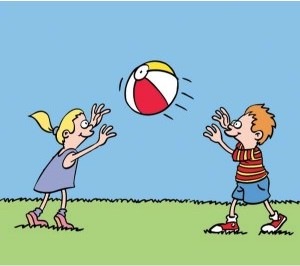
\includegraphics[width=0.25\columnwidth]{figures/I21.jpg}} \\
\hline
What is the girl doing? & What is the boy doing? & What is the boy doing? \\
\hline
\end{tabular}
%\caption{\label{tab:example-pdt-items} PDT example images with their targeted questions. In the untargeted form, the question for each is \textit{What is happening?} From left to right, the examples represent one intransitive, transitive and ditransitive item.}
\end{center}
\end{table}
\medskip
\end{frame}

\begin{frame}
\frametitle{Recap: Feature annotation}
\begin{table}[htb!]
\scriptsize
\begin{center}
%\begin{tabular}{|p{3.7cm}|c|c|c|c|c|}
\begin{tabular}{|l|c|c|c|c|c|}
\hline
\multicolumn{6}{|c|}{
\includegraphics[width=0.3\columnwidth]{figures/I02.jpg}} \\
\hline
\textit{What is the boy doing?} & C & A & G & I & V \\
\hline
\hline
He is eating food. & 0 & 1 & 1 & 1 & 1 \\
\hline
he eating. & 0 & 1 & 0 & 1 & 1 \\
\hline
The child is about to eat pizza. & 1 & 0 & 1 & 1 & 1 \\
\hline
He may get fat eating pizza. & 0 & 0 & 1 & 1 & 0 \\
\hline
\end{tabular}
\caption{\label{tab:dev-transitive} \scriptsize Annotated for five features: Core event (\textit{C}), Answerhood (\textit{A}), Grammaticality (\textit{G}), Interpretability (\textit{I}) and Verifiability (\textit{V}).}
\end{center}
\end{table}

\end{frame}

\begin{frame}
\frametitle{Recap: Feature annotation weights}
\scriptsize
I used a preference test to establish feature weights. In this toy example, weights are based on 3 pairs. The net score for the preferred responses for each feature is divided by the sum of all 5 net scores (sum$=$6; e.g., \textit{C} weight: 2/6$=$.333). The real weights$^*$ are based on 1200 pairs across all items.
\begin{table}
\scriptsize
\begin{center}
\begin{tabular}{|=l|+c||+c|+c|+c|+c|+c|}
\hline
\textit{What is the boy doing?} & Pref? & C & A & G & I & V \\
\hline
\multicolumn{7}{c}{} \\
\hline
\rowstyle{\color{OliveGreen}}He is eating food. & \textbf{yes} & \textbf{0} & \textbf{1} & \textbf{1} & \textbf{1} & \textbf{1} \\
\hline
\rowstyle{\color{Maroon}}He may get fat eating. & no & 0 & 0 & 1 & 1 & 0 \\
\hline
\multicolumn{7}{c}{} \\
\hline
\rowstyle{\color{Maroon}}He is hungry. & no & 0 & 0 & 1 & 0 & 1 \\
\hline
\rowstyle{\color{OliveGreen}}the boy is eating pizza & \textbf{yes} & \textbf{1} & \textbf{1} & \textbf{1} & \textbf{1} & \textbf{1} \\
\hline
\multicolumn{7}{c}{} \\
\hline
\rowstyle{\color{OliveGreen}}The child is about to eat pizza. & \textbf{yes} & \textbf{1} & \textbf{0} & \textbf{1} & \textbf{1} & \textbf{1} \\
\hline
\rowstyle{\color{Maroon}}he eating. & no & 0 & 1 & 0 & 1 & 1 \\
\hline
\multicolumn{7}{c}{} \\
\hline
\rowstyle{\color{OliveGreen}}Totals preferred responses & & 2 & 2 & 3 & 3 & 3 \\
\hline
\rowstyle{\color{Maroon}}Totals dispreferred responses & & 0 & 1 & 2 & 2 & 2 \\
\hline
\rowstyle{\color{OliveGreen}}Net preferred (pref {\color{black}-} {\color{Maroon}dispref}) & & 2 & 1 & 1 & 1 & 1 \\
\hline
Feature weight &  & .333 & .167 & .167 & .167 & .167 \\
\hline
\multicolumn{7}{c}{} \\
\hline
$^*$Real feature weight &  & .365 & .093 & .055 & .224 & .263 \\
\hline
\end{tabular}
%\caption{\label{tab:dev-transitive} \scriptsize Annotated for five features: Core event (\textit{C}), Verifiability (\textit{V}), Answerhood (\textit{A}), Interpretability (\textit{I}) and Grammaticality (\textit{G}).}
\end{center}
\end{table}

\end{frame}

\begin{frame}
\frametitle{Recap: Gold Standard}
\scriptsize
I applied the feature weights to the annotations to establish a gold standard (GS) score for each NNS response (n=70) for each PDT item. I ranked by GS score to get a GS ranking. (I use the real weights in this example.)
\begin{table}
\tiny
%\begin{table}[t!] This line is giving me trouble when I go to typeset
\begin{center}
%\begin{tabular}{|p{3.7cm}|c|c|c|c|c|}
\begin{tabular}{|l|l|c|c|c|c|c||l|c|}
%\hline
%\multicolumn{6}{|c|}{
\includegraphics[width=0.45\columnwidth]{figures/I02.jpg}} \\
%\multicolumn{6}{|c|}{
\includegraphics[width=0.3\columnwidth]{figures/I02.jpg}} \\
\hline
%\multicolumn{3}{|l|}{What is the woman doing? [Intransitive]} \\
Participant & \textit{What is the boy doing?} & C & A & G & I & V & \tiny{GS score} & \tiny{GS rank} \\
\hline
p1 & The boy is eating. & 0 & 1 & 1 & 1 & 1 & 0.635 & 4 \\
\hline
p2 & A baby is eating pizza & 0 & 0 & 1 & 1 & 0 & 0.279 & 5 \\
\hline
p3 & The boy enjoys his pizza. & 1 & 0 & 1 & 1 & 1 & 0.907 & 2 \\
\hline
p4 & the boy is eating pizza & 1 & 1 & 1 & 1 & 1 & 1.0 & 1 \\
\hline
p5 & The kid is eats pizza & 1 & 0 & 0 & 1 & 1 & 0.852 & 3 \\
\hline
\end{tabular}
%\caption{\label{tab:dev-transitive} \scriptsize Annotated for five features: Core event (\textit{C}), Verifiability (\textit{V}), Answerhood (\textit{A}), Interpretability (\textit{I}) and Grammaticality (\textit{G}).}
\end{center}
\end{table}

\end{frame}

\begin{frame}
\frametitle{Recap: Auto scoring}
\scriptsize
I have a system for automatically scoring the NNS responses. (The details aren't really important here, but ...)
\bigskip

For each item, the process is like this:

For the collection of NS responses  (n=50 per PDT item):

1) dependency parse;

2) get tf-idf score for each unique dependency (\textit{Compare against a large balanced corpus; common dependencies get low scores, rare dependencies get higher scores}).
\bigskip

For each NNS response, repeat \textit{1} and \textit{2}, then compare NS vs NNS (dependency scores vectors) -- use cosine. This is the NNS response score.

\bigskip

By selecting different parameters in this approach, I arrive at 12 different system configurations. Each configuration scores and ranks all NNS responses (n=70).

\end{frame}

\begin{frame}
\frametitle{Recap: Configurations}
\scriptsize

Rather than the full set of 12 configurations, let's consider this simplified set of 2 parameters $x$ 2 settings $=$ 4 configurations.
\medskip

\textbf{Parameters}:
\scriptsize
\begin{itemize}
\item \textbf{Dependency format}:
\begin{itemize}
\item \textbf{labeled}: e.g., nsubj(eat,boy); nobj(eat,pizza)
\item \textbf{unlabeled}: e.g., $\langle$null$\rangle$(eat,boy); $\langle$null$\rangle$(eat,pizza)
\end{itemize}
\item \textbf{NS response model}:
Each NS participant gave \textit{two} responses per PDT item
\begin{itemize}
\item \textbf{first}: Model contains only the first response from NS (n=50)
\item \textbf{mixed}: Model is half first reponses (n=25) and half second responses (n=25)
\end{itemize}
\end{itemize}
\begin{table}[htb!]
\scriptsize
\begin{center}
%\begin{tabular}{|p{3.7cm}|c|c|c|c|c|}
\begin{tabular}{|l|l|l|}
\hline
dep\textbackslash model & first & 1st \& mixed \\
\hline
labeled & lab\_first & lab\_mixed \\
\hline
unlabeled & unlab\_first & unlab\_mixed \\
\hline
\end{tabular}
\caption{\scriptsize Four system configurations for scoring NNS responses.}
\end{center}
\end{table}

\end{frame}


\begin{frame}
\frametitle{Recap: Gold Standard}
\scriptsize
I run the NNS responses through my system using the four different configurations. This yields a score and ranking for each response.
\begingroup
\setlength{\tabcolsep}{4pt} % Default value: 6pt
\begin{table}
\tiny
\begin{center}
\begin{tabular}{|l||c|c|c|c|c||l|c||l|c||l|c||l|c||l|c|}
\hline
P & C & A & G & I & V & \tiny{GS s} & \tiny{GS r} & \tiny{lf s} & \tiny{lf r} & \tiny{uf r} & \tiny{uf r} & \tiny{lm s} & \tiny{lm r} & \tiny{um r} & \tiny{um r} \\
\hline
p1 & 0 & 1 & 1 & 1 & 1 & 0.63 & 4 & .53 & 4 & .11 & 5 & 0.29 & 4 & .39 & 3 \\
\hline
p2 & 0 & 0 & 1 & 1 & 0 & 0.27 & 5 & .13 & 5 & .15 & 4 & 0.15 & 5 & .53 & 5 \\
\hline
p3 & 1 & 0 & 1 & 1 & 1 & 0.90 & 2 & .91 & 1 & .68 & 1 & 0.33 & 3 & .55 & 1 \\
\hline
p4 & 1 & 1 & 1 & 1 & 1 & 1.0 & 1 & .80 & 2 & .41 & 2 & 0.70 & 1 & .24 & 2 \\
\hline
p5 & 1 & 0 & 0 & 1 & 1 & 0.85 & 3 & .77 & 3 & .20 & 3 & 0.63 & 2 & .22 & 4 \\
\hline
\end{tabular}
\caption{\label{tab:modelranks} \scriptsize Response scores (\textit{s}) and ranks (\textit{r}) for: gold standard (\textit{GS}); four configurations: labeled\_first (\textit{lf}), unlabeled\_first (\textit{uf}), labeled\_mixed (\textit{lm}), unlabeled\_mixed (\textit{um}).}
\end{center}
\end{table}
\endgroup
\end{frame}

\begin{frame}
\frametitle{Stats questions}
\scriptsize
That brings us to where I'm stuck...

\begin{itemize}
\item I have three basic categories of PDT item -- \textbf{intransitive, transitive, ditransitive}. (There is some variation, e.g., \textit{She is riding a bike} vs. \textit{She is bicycling}, but these categories are roughly true.)
\item Ideally, I'd like to \textbf{find trends} that allow me to \textbf{optimize my configuration} for each item category.

\item What I've tried:

\item I used the GS ranking and the configuration rankings to calculate a single \textbf{Spearman} correlation for each configuration, for each item.
\item 12 configurations $x$ 30 items $=$ 360 Spearman scores.
\item I used these scores to generate hierarchical clusters of items. I did this in nearly every conceivable way; I used: \textit{all} items; \textit{individual} items; I averaged Spearman scores for a given parameter setting, e.g., to compare labeled and unlabeled, I averaged \textit{labeled\_first} $+$ \textit{labeled\_mixed}, then averaged \textit{unlabeled\_first} $+$ \textit{unlabeled\_mixed}, then clustered items based on these two sets of values.
\item I hoped to find intransitive items clustered together, transitive items clustered together, etc. Any such trends appear very weak, however.

\end{itemize}

\end{frame}


\begin{frame}
\frametitle{Stats questions}
\scriptsize
\begin{itemize}
\item I need guidance on to how to approach this in a sound way.

\item I've begun experimenting with \textbf{T-test} and \textbf{Wilcox} test. In this case, the idea is to analyze individual features. For example, for a given item and for a given configuration, group all responses where \textit{Core event} is annotated ``1'', then group all the ``0'' responses. Then run a \textbf{paired sample T-test} using the system score for those groups to see if there are significant differences between them. If I do this for all items, I can look for differences between the intransitive, transitive, ditransitive items across all configurations.
\item An important note here -- the \textbf{feature annotations are heavily skewed}. For a handful of the (30 items $x$ 5 features $=$) 150 cases, a feature is ``1'' for \textit{all} responses.

\item I'm also considering this approach but using \textbf{average precision} instead of T-test. In this case, I'd be looking for configurations that maximize the separation of ``0'' and ``1'' responses.


\end{itemize}

\end{frame}
%\section{Related Work}
%\begin{frame}
%\frametitle{Related Work}
%
%\begin{itemize}
%\item \textit{Herr Komissar}: ILT/detective game for German learners, includes
%content analysis \& sentence generation \citep{desmedt:95}, but
%uses many custom-built tools. 
%\item \citet{petersen:10}: ILT, provides feedback on questions in English,
%extracting meanings from an existing parser.
%\item Content assessment: (e.g., ETS's c-rater system \citep{leacock:chodorow:03}); mostly focused on essay \& short answer scoring. 
%	\begin{itemize}
%	\item Some focus on semantic analysis under restricted conditions, e.g., \citep{Meurers.Ziai.ea-11}.
%%evaluate English language learners' short
%%answers to reading comprehension questions, constrained by topic
%%at hand; system performs annotation (on reading, question \& response), including dependency parsing \& lexical analysis.
%%(WordNet \citep{Fellbaum:1998}), aligns elements of the
%%response with those of (similarly annotated) reading prompt,
%%question, and target answers to determine if response is
%%adequate or what is missing.
%
%	\end{itemize}
%\end{itemize}
%
%\end{frame}
%
%\section{Data Collection}
%\begin{frame}
%\frametitle{Data Collection}
%We use a picture description task (PDT) because:
%\begin{itemize}
%\item Computer games/ILTs are visual.
%\item Visual prompts restrict response contents to image contents.
%\item Responses model real language use and are pure interlanguage-- no influence of verbal prompts.
%\end{itemize}
%Our PDT:
%\begin{itemize}
%\item We chose 10 images depicting transitive events (unambiguous subject, verb, object) to restrict form in addition to content.
%\item Participants were instructed to view the image \& describe the action in one sentence; past or present tense
%(and simple or progressive aspect) were accepted.
%\end{itemize}
%% example is given in Figure~\ref{fig:example-picture}. 
%\end{frame}
%
%\begin{frame}
%\frametitle{Data Collection}
%\framesubtitle{Example item and responses}
%\footnotesize
%\begin{figure}[width=0.8\columnwidth]
%\begin{center}
%\begin{tabular}{|c|}
%\hline
%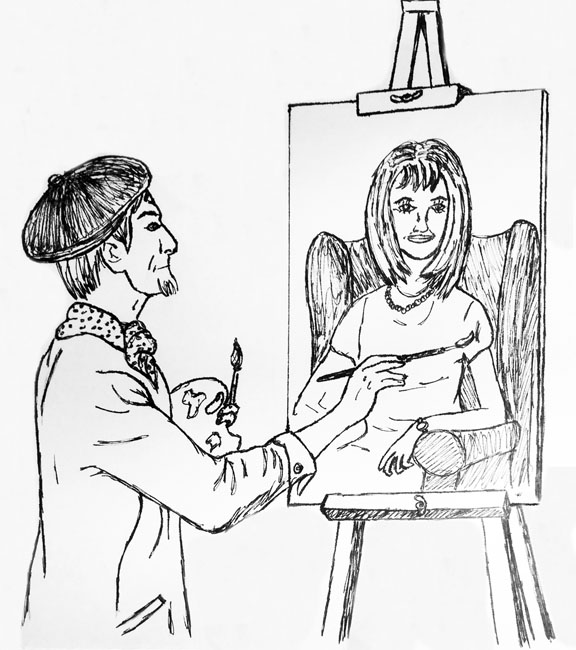
\includegraphics[width=0.5\columnwidth]{figures/exampleprompt.jpg}\\
%\hline
%\textbf{Response (L1)}\\
%\hline
%He is droning his wife pitcher. (Arabic)\\
%\hline
%The artist is drawing a pretty women. (Chinese) \\
%\hline
%The artist is painting a portrait of a lady. (English) \\
%\hline
%The painter is painting a woman's paint. (Spanish)\\
%\hline
%\end{tabular}
%\end{center}
%% \caption{Example item and responses}
%% \label{fig:example-picture}
%\end{figure}
%\end{frame}
%
%\begin{frame}
%\frametitle{Data Collection}
%\framesubtitle{Participants}
%
%% MD: *the* Intensive English Program?
%53 Participants: 14 NS, 39 NNS. The NNS consisted of:
%\begin{itemize}
%\item intermediate \& upper-level adult learners enrolled in the IU Intensive English Program. 
%\item 16 Arabic, 7 Chinese, 2 Japanese, 4 Korean, 1 Kurdish, 1 Polish, 2 Portuguese, 6 Spanish.
%\end{itemize}
%\end{frame}
%
%
%\section{Method}
%\begin{frame}
%\frametitle{Method}
%
%%We:
%\begin{enumerate}
%\item Parse a sentence into a dependency representation 
%\item Extract a simple semantic form from this parse
%\begin{itemize}
%\item to compare to gold standard semantic forms
%\end{itemize}
%\end{enumerate}
%
%\end{frame}
%
%\subsection{Syntactic form}
%\begin{frame}
%\frametitle{Obtaining a syntactic form}
%Dependency parsing:
%\begin{itemize}
%\item labels dependency relations, not phrase structure;
%\item easily finds a sentence's subject, verb and object;
%\end{itemize}
%For transitive sentences, we consider S,V,O as adequate (for now) for evaluating whether sentence describes image.
%
%%Eventually, we need to account for other relations, e.g., negation, adverbial modification. \\
%
%\medskip
%
%We use the Stanford Parser for this task:
%\begin{itemize}
%\item trained on the Penn Treebank;
%\item use Stanford typed dependency labels;
%\item {\tt CCPropagatedDependencies} / {\tt CCprocessed} options:
%	\begin{enumerate}
%	\item propagate dependencies across conjunctions;
%	\item omit prepositions \& conjunctions from sentence text; add them to dependency label between content words
%	\end{enumerate}
%\end{itemize}
%\end{frame}
%
%\begin{frame}[t]{Top alignment}
%\frametitle{Stanford Parser settings}
%%\begin{center}
%\begin{tabular}{|c|}%[width=0.55\columnwidth]
%\hline
%\begin{dependency}[arc edge,text only label,label style={above}]
%\begin{deptext}[column sep=.3em]
%  \textit{vroot} \& The \&[1em] boy \&[1em] and \& girl \& played \& with \& the \& ball \\
%  				\& DT \& NN \& CC \& NN \& VBD \& IN \& DT \& NN \\
%\end{deptext}
%\depedge[arc angle=90]{1}{6}{root}
%\depedge{3}{2}{det}
%\depedge[arc angle=35]{3}{4}{cc}
%\depedge[arc angle=80]{3}{5}{conj}
%\depedge[arc angle=90]{6}{3}{nsubj}
%\depedge{6}{7}{prep}
%\depedge[arc angle=90]{7}{9}{pobj}
%\depedge{9}{8}{det}
%%    \depedge[edge style={gray,very thick},label style={text=gray}]{3}{6}{prep\_with}
%\end{dependency} \\
%Basic format \\
%\hline
%\begin{dependency}[arc edge,text only label,label style={above}]
%\begin{deptext}[column sep=.3em]
%  \textit{vroot} \& The \&[1em] boy \&[1em] and \& girl \& played \& with \& the \& ball \\
%  				\& DT \& NN \& CC \& NN \& VBD \& IN \& DT \& NN \\
%\end{deptext}
%\depedge[arc angle=90]{1}{6}{root}
%\depedge{3}{2}{det}
%\depedge[arc angle=90]{6}{3}{nsubj}
%\depedge[edge style={very thick},label style={font=\bfseries,thick},arc angle=35]{6}{5}{nsubj}
%%    \depedge[edge style={very thick}]{6}{5}{nsubj}
%\depedge[edge style={very thick},label style={font=\bfseries,thick},arc angle=90]{6}{9}{prep\_with}
%\depedge{9}{8}{det}
%
%\end{dependency} \\
%With {\tt CCPropagatedDependencies} / {\tt CCprocessed} options \\
%\hline
%\end{tabular}
%%\end{center}
%\end{frame}
%
%\subsection{Semantic form}
%\begin{frame}
%\frametitle{Obtaining a semantic form}
%\begin{itemize}
%\item We categorized sentences into 12 types, each corresponding to a basic sentence structure. \\
%\item The type indicates that the logical S,V,O are found under particular labels, indices or POS tags. \\
%\item Distributions for the most common types are shown below; expletive types are omitted here. \\
%\end{itemize}
%\begin{table}[width=.8\columnwidth]
%\scriptsize
%\begin{center}
%\begin{tabular}{|c|l|l|r|r|}
%\hline
%\textbf{{\tiny Type}} & \textbf{Description} & \textbf{Example} & NS & NNS \\
%\hline
%A & Simple declar. trans. & The boy is kicking the ball. & 117 & 286 \\
%\hline
%B & Simple + preposition & The boy played with a ball. & 5 & 23 \\
%\hline
%C & Missing tensed verb & Girl driving bicycle. & 10 & 44 \\
%\hline
%D & Missing tensed V + prep & Boy playing with a ball. & 0 & 1 \\
%\hline
%E & Intransitive (No object) & A woman is cycling. & 2 & 21 \\
%\hline
%F1 & Passive & An apple is being cut. & 4 & 2 \\
%\hline
%F2 & Passive with agent & A bird is shot by a man. & 0 & 6 \\
%\hline
%Z & All other forms & The man is trying to... & 2 & 6 \\
%\hline
%\end{tabular}
%\end{center}
%%\caption{Sentence type examples, with distributions of types for
%%  native speakers (NS) and non-native speakers (NNS)}
%\label{tab:sentence-type}
%\end{table}
%\end{frame}
%
%\begin{frame}
%\frametitle{Sentence types}
%%\begin{itemize}
%%\item 
%We use type features to construct a binary decision tree for determining type.
%
%\begin{figure}
%\footnotesize
%\begin{center}
%\begin{tikzpicture}
%% MD: I think in the future we could put something like (p. 3 of manual):
%% \tikzset{every internal node/.style={font=\tt}}
%\tikzset{level distance=3.5em}
%\tikzset{edge from parent/.append style={->}}
%\Tree
%[.{\tt expl}?
%\edge node[auto=right,pos=.6,inner sep=1pt]{Y};
%[.{\tt auxpass}? 
%	\edge node[auto=right,pos=.6,inner sep=1pt]{Y};
%	[.{\tt agent}? 
%		\edge node[auto=right,pos=.6,inner sep=1pt]{Y};
%		[.F2x ]
%		\edge node[auto=left,pos=.6,inner sep=1pt]{N};
%		[.F1x ]
%	]
%	\edge node[auto=left,pos=.6,inner sep=1pt]{N};
%	[.{\tt dobj}? 
%		\edge node[auto=right,pos=.6,inner sep=1pt]{Y};
%		[.Ax ]
%		\edge node[auto=left,pos=.6,inner sep=1pt]{N};
%		[.{\tt prep\_}$\ast$?
%			\edge node[auto=right,pos=.6,inner sep=1pt]{Y};
%			[.Bx ]
%			\edge node[auto=left,pos=.6,inner sep=1pt]{N};
%			[.Ex ]
%		]
%	]
%]
%\edge node[auto=left,pos=.6,inner sep=1pt]{N};
%[.{\tt nsubjpass}? 
%	\edge node[auto=right,pos=.6,inner sep=1pt]{Y};
%	[.{\tt agent}? 
%		\edge node[auto=right,pos=.6,inner sep=1pt]{Y};
%		[.F2 ]
%		\edge node[auto=left,pos=.6,inner sep=1pt]{N};
%		[.F1 ]
%	]
%	\edge node[auto=left,pos=.6,inner sep=1pt]{N};
%	[.{\tt dobj}? 
%		\edge node[auto=right,pos=.6,inner sep=1pt]{Y};
%		[.{\tt nsubj}?
%			\edge node[auto=right,pos=.6,inner sep=1pt]{Y};
%			[.A ]
%			\edge node[auto=left,pos=.6,inner sep=1pt]{N};
%			[.C ]
%		]
%		\edge node[auto=left,pos=.6,inner sep=1pt]{N};
%		[.{\tt nsubj}?
%			\edge node[auto=right,pos=.6,inner sep=1pt]{Y};
%			[.{\tt prep\_}$\ast$?
%			 	\edge node[auto=right,pos=.6,inner sep=1pt]{Y};
%				[.B ]
%				\edge node[auto=left,pos=.6,inner sep=1pt]{N};
%				[.E ]
%			]
%%				\edge node[auto=right,pos=.6,inner sep=1pt]{Y};
%%				[.B ]
%			\edge node[auto=left,pos=.6,inner sep=1pt]{N};
%			[.D ]
%			]
%%			\edge node[auto=left,pos=.6,inner sep=1pt]{N};
%%			[.D
%%			]
%		]
%	]
%]
%]
%\end{tikzpicture}
%\end{center}
%%\caption{Decision tree for determining sentence type and extracting semantic information}
%\label{fig:decision-tree}
%\end{figure}
%\end{frame}
%
%\begin{frame}
%\frametitle{Rules for sentence types}
%\begin{itemize}
%\item Each type has a set of rules for extracting semantic triples in the form \textit{verb(subj,obj)}. \\
%\item For type B, for example, we extract the {\tt root} as verb and {\tt nsubj} as subject. The object is taken from {\tt prep\_}$\ast$, provided it is a dependent of the root. \\
%\item For the example below, we extract \textit{played(boy,ball)}. \\
%\end{itemize}
%\begin{figure}
%\begin{center}
%\begin{dependency}[arc edge,text only label,label style={above}]
%\begin{deptext}[column sep=.5em]
%  \textit{vroot} \& The \&[1em] \textbf{boy} \&[1em] \textbf{played} \& with \& a \&[1em] \textbf{ball} \\
%\end{deptext}
%\depedge[label style={font=\bfseries,thick}]{4}{3}{nsubj}
%\depedge[arc angle=90,label style={font=\bfseries,thick}]{1}{4}{root}
%%    \depedge[edge style={gray,very thick},label style={text=gray}]{3}{6}{prep\_with}
%\depedge[label style={font=\bfseries,thick}]{4}{7}{prep\_with}
%\depedge[arc angle=35]{7}{6}{det}
%\depedge{3}{2}{det}
%\end{dependency}
%\end{center}
%\label{fig:prep-dependency}
%\end{figure}
%
%\end{frame}
%
%\section{Evaluation}
%\begin{frame}
%\frametitle{Evaluation}
%\textbf{Two major questions for evaluation:}
%\begin{enumerate}
%\item How accurately do we extract semantic information from potentially innovative sentences? \\
%\item How many semantic forms do we need in order to capture the variability in learner sentences? \\
%	\begin{itemize}
%	\item How well does the set of native speaker forms model a gold standard? \\
%	\end{itemize}
%\end{enumerate}
%\end{frame}
%
%%\subsection{Sentence distribution}
%%\begin{frame}
%%\frametitle{Basic distribution of sentences}
%%
%%\end{frame}
%
%\subsection{Semantic extraction}
%\begin{frame}
%\frametitle{Semantic extraction}
%
%To evaluate our extraction system, we define two classes of errors:
%\begin{enumerate}
%\item \textit{triple errors}: system fails to extract one or more of
%the desired subject, verb, or object
%\begin{itemize}
%\item No regard to target content
%\end{itemize}
%\item \textit{content errors}: system extracts the desired triple, but
%the triple does not accurately describe the image
%%(i.e., is an error of the participant's)
%\end{enumerate}
%
%%\medskip
%
%\end{frame}
%
%%\begin{frame}
%%\frametitle{Error subcategorization}
%%
%%% MD: may not need this slide, if you can talk through following one
%%
%%Triple error subcategorization:
%%\begin{itemize}
%%\item \textit{Speaker}: typically misspellings in the original
%%  sentence, leading to an incorrect POS tag \& parse
%%\item \textit{Parser}: a correct sentence parsed incorrectly or in a
%%  way to indicate a different meaning from the one intended
%%  %; an example is given in the figure.
%%\item \textit{Extraction}: failure of the extraction script to find
%%  one or more of the desired subject, verb or object
%%  % \begin{itemize}
%%  % \item Typically involve more complex sentence structures, such as
%%  %   conjoined or embedded clauses
%%  % \end{itemize}
%%\end{itemize}
%%
%%\medskip
%%
%%Content error subcategorization:
%%\begin{itemize}
%%\item \textit{Spelling}: triple word misspelled severely enough that
%%  intended spelling cannot be discerned
%%  \begin{itemize}
%%  \item Do not result in downstream errors, i.e., have well-formed
%%    triples except for misspelled target word(s)
%%  \end{itemize}
%%
%%\item \textit{Meaning}: inaccurate word within the triple
%%  \begin{itemize}
%%  \item Include misspellings resulting in real but unintended word
%%    (e.g., \textit{shout(man,bird)} vs.  \textit{shoot(man,bird)})
%%  \end{itemize}
%%\end{itemize}
%%
%%\end{frame}
%%
%
%\begin{frame}
%\frametitle{Triple errors}
%
%\begin{table}[htb!]
%\begin{center}
%\scriptsize
%% reduce space between columns
%%\setlength{\tabcolsep}{.3em}
%\begin{tabular}{|l|p{10em}c|r|}
%\hline
%& \multicolumn{2}{c|}{Example} &  \\
%Error type & Sentence & Triple & Count (\%)\\
%\hline
%\hline
%\multicolumn{4}{c}{}\\
%\multicolumn{4}{c}{\textbf{NNS}} \\
%\hline
%Speaker & A man swipped leaves. & leaves(swipped,man) & 16 (4.1\%) \\
%\hline
%Parser & Two boys boat. & NONE(boys,NONE) & 5 (1.3\%) \\
%\hline
%Extraction & A man is gathering lots of leafs. & gathering(man,lots) & 9 (2.3\%) \\
%\hline
%\textbf{Total} (390) & & & \textbf{30 (7.7\%)} \\
%% \cmidrule{2-6}\morecmidrules\cmidrule{2-6}
%\hline
%\multicolumn{4}{c}{}\\
%\multicolumn{4}{c}{\textbf{NS}} \\
%\hline
%Speaker & (\textit{None}) & & 0 (0\%) \\
%\hline
%Parser & An old man raking leaves on a path. & leaves(man,path) & 2 (1.4\%) \\
%\hline
%Extraction & A man has shot a bird that is falling from the sky. & shot(bird,sky) & 8 (5.7\%) \\
%\hline
%\textbf{Total} (140) & & & \textbf{10 (7.1\%)} \\
%\hline
%\end{tabular}
%\end{center}
%% \caption{Triple errors and content errors by subcategory, with error
%%   rates reported (e.g., 7.7\% error = 92.3\% accuracy)}
%% \label{tab:error-types}
%\end{table}
%
%\end{frame}
%
%\begin{frame}
%\frametitle{Parser error example}
%
%%\begin{figure}[htb!]
%\begin{center}
%\begin{tabular}{|c|}
%\hline
%Actual parse and resulting triple \\
%\hline
%\begin{dependency}[arc edge,text only label,label style={above}]
%\begin{deptext}[column sep=.5em]
%  \textit{vroot} \& Two \&[1em] boys \&[1em] boat \\
%  				\&	CD \&	NNS		\&	NN	\\
%\end{deptext}
%\depedge{3}{2}{num}
%\depedge[arc angle=90]{1}{3}{root}
%%    \depedge[edge style={gray,very thick},label style={text=gray}]{3}{6}{prep\_with}
%\depedge{3}{4}{dep}
%\end{dependency} \\
%NONE(boys,NONE) \\
%\hline
%\end{tabular}
%\end{center}
%
%
%\begin{center}
%\begin{tabular}{|c|}
%\hline
%Desired parse and triple \\
%\hline
%\begin{dependency}[arc edge,text only label,label style={above}]
%\begin{deptext}[column sep=.5em]
%  \textit{vroot} \& Two \&[1em] boys \&[1em] boat \\
%  				\&	CD \&	NNS		\&	VBP	\\
%\end{deptext}
%\depedge{3}{2}{num}
%\depedge{1}{4}{root}
%%    \depedge[edge style={gray,very thick},label style={text=gray}]{3}{6}{prep\_with}
%\depedge{4}{3}{nsubj}
%\end{dependency} \\
%boat(boys,NONE) \\
%\hline
%\end{tabular}
%\end{center}
%% \caption{A parser error leading to a triple error (top), and the
%%   desired parse and triple (bottom).}
%% \label{fig:parser-error}
%%\end{figure}
%
%\end{frame}
%
%\begin{frame}
%\frametitle{Content errors}
%
%\begin{table}[htb!]
%\begin{center}
%\scriptsize
%% reduce space between columns
%\setlength{\tabcolsep}{.5em}
%\begin{tabular}{|l|p{10em}c|r|}
%\hline
%& \multicolumn{2}{c|}{Example} &  \\
%Error type & Sentence & Triple & Count (\%)\\
%\hline
%\hline
%\multicolumn{4}{c}{}\\
%\multicolumn{4}{c}{\textbf{NNS}} \\
%\hline
%Spelling & The artiest is drawing a portret. & drawing(artiest,portret) & 36 (9.2\%) \\
%\hline
%Meaning & The woman is making her laundry. & making(woman,laundry) & 23 (5.9\%) \\
%\hline
%\textbf{Total} (390) & & & \textbf{59 (15.1\%)} \\
%% \cmidrule{2-6}\morecmidrules\cmidrule{2-6}
%\hline
%
%\multicolumn{4}{c}{}\\
%\multicolumn{4}{c}{\textbf{NS}} \\
%\hline
%Spelling & (\textit{None}) & & 0 (0\%) \\
%\hline
%Meaning & A picture is being taken of a girl on a bike. & taken(NONE,picture) & 3 (2.1\%) \\
%\hline
%\textbf{Total} (140) & & & \textbf{3 (2.1\%)} \\
%\hline
%\end{tabular}
%\end{center}
%% \caption{Triple errors and content errors by subcategory, with error
%%   rates reported (e.g., 7.7\% error = 92.3\% accuracy)}
%% \label{tab:error-types}
%\end{table}
%
%\end{frame}
%
%%\begin{frame}
%%\frametitle{Semantic extraction}
%%\framesubtitle{Analysis}
%%
%%Extraction for NNS/NS data:  92.3\%/92.9\% accuracy
%%\begin{itemize}
%%\item Many errors for NSs stem from extractor, due to native speakers
%%  using more complex structures.  
%%\item Many errors for NNSs involve misspellings
%%  \begin{itemize}
%%  \item For a system interacting with learners, spelling errors are
%%    thus more of a priority \citep[cf.][]{hovermale:08}
%%  \end{itemize}
%%\end{itemize}
%%
%%\medskip
%%
%%% Goal of a system: identify the 15.1\% of NNS sentences which are
%%% content errors, in order to provide feedback.  
%%% \begin{itemize}
%%% \item 7.7\% triple errors would also be grouped into this set\\
%%%   $\Rightarrow$ need further extraction improvements
%%% \end{itemize}
%%
%%Minor point: three content errors among NS responses
%%\begin{itemize}
%%\item Meta-description of image prompt rather than a direct
%%  description of image contents
%%\item e.g., \textit{A picture is being taken of a girl on a bike}
%%  vs. \textit{A girl is riding a bike}
%%\end{itemize}
%%
%%\end{frame}
%
%\subsection{Semantic coverage}
%\begin{frame}
%\frametitle{Semantic coverage}
%Idea: Treat NS set as gold standard.
%
%\medskip
%
%Pre-processing:
%\begin{itemize}
%\item Manually removed \textit{triple} errors from set of NNS triples
%\item Manually removed \textit{all} errors from set of NS triples
%\item Lemmatized: \textit{rowed(boys,boat)} $\Rightarrow$ \textit{row(boy,boat)}
%\end{itemize}
%
%\medskip
%
%Evaluation:
%\begin{itemize}
%%\item Compared NS \& NNS triples
%%\item Main idea: Of semantically appropriate NNS triples, how many occur in NS set?
%\item Coverage: Measure of how many ``good" NNS responses are found in NS data
%\item Accuracy: Measure of how many ``good" NNS responses are found in NS data + how many ``bad" NNS responses are \textit{not} found in NS data
%\end{itemize}
%\end{frame}
%
%\begin{frame}
%\frametitle{Semantic triple matching}
%%\framesubtitle{\emph{NS}/\emph{NNS}: number of unique triples for NSs/NNSs}
%
%%\begin{table}[htb!]
%\begin{center}
%% reduce space between columns
%\setlength{\tabcolsep}{.5em}
%\begin{tabular}{|c||cc|cc|}
%\hline
%& \multicolumn{2}{c|}{Coverage} & \multicolumn{2}{c|}{Accuracy}\\
%Item & Type & Token & Type & Token\\
%\hline
%\hline
%1 & 3/12 & 23/38 & 5/14 & 25/39 \\
%\hline
%2 & 3/9 & 15/28 & 8/14 & 20/32 \\
%\hline
%3 & 5/12 & 23/30 & 12/19 & 30/36 \\
%\hline
%4 & 2/6 & 32/37 & 4/8 & 34/39 \\
%\hline
%5 & 1/16 & 3/25 & 9/24 & 11/33 \\
%\hline
%6 & 3/17 & 16/31 & 8/22 & 21/36 \\ %16/32 --> 16/31, 21/37 --> 21/36
%\hline
%7 & 5/19 & 14/35 & 9/23 & 18/39 \\
%\hline
%8 & 5/16 & 10/30 & 11/22 & 17/36 \\
%\hline
%9 & 3/21 & 3/23 & 15/33 & 15/35 \\
%\hline
%10 & 2/8 & 14/24 & 15/21 & 27/35 \\
%\hline
%\hline
%Total & \textbf{32/136} & \textbf{153/301} & \textbf{96/200} & \textbf{218/360}\\
%  & \textbf{23.5\%} & \textbf{50.8\%} & \textbf{48.0\%} & \textbf{60.6\%}\\
%\hline
%\end{tabular}
%\end{center}
%
%\end{frame}
%
%\begin{frame}
%\frametitle{Variability of forms: single PDT item}
%\framesubtitle{Italics = not in NSs, but could be inferred}
%
%%\begin{table}[htb!]
%\begin{center}
%\footnotesize
%\begin{tabular}{|l|c|c|c|}
%\hline
%Type & NNS & NS & Coverage \\
%\hline
%\hline
%\textit{cut(woman,apple)} & \textit{5} & \textit{0} & \textit{(5)} \\
%\hline
%cut(someone,apple) & 4 & 2 & 4 \\
%\hline
%cut(somebody,apple) & 3 & 0 & \\
%\hline
%cut(she,apple) & 3 & 0 & \\
%\hline
%slice(someone,apple) & 2 & 5 & 2 \\
%\hline
%cut(person,apple) & 2 & 1 & 2\\
%\hline
%\textit{cut(NONE,apple)} & \textit{2} & \textit{0} & \textit{(2)} \\
%\hline
%slice(woman,apple) & 1 & 1 & 1 \\
%\hline
%slice(person,apple) & 1 & 1 & 1 \\
%\hline
%slice(man,apple) & 1 & 0 & \\
%\hline
%cut(person,fruit) & 1 & 0 & \\
%\hline
%cut(people,apple) & 1 & 0 & \\
%\hline
%cut(man,apple) & 1 & 0 & \\
%\hline
%cut(knife,apple) & 1 & 0 & \\
%\hline
%chop(woman,apple) & 1 & 0 & \\
%\hline
%chop(person,apple) & 1 & 0 & \\
%\hline
%slice(NONE,apple) & 0 & 2 & \\
%\hline
%Total  &  30 & 12 & 10 \textit{(17)} \\
%\hline
%\end{tabular}
%\end{center}
%% \caption{Distribution of valid tokens across types for a single PDT item. Types in italics do not occur in the NS sample, but could be inferred to expand coverage by recombining elements of NS types that do occur.}
%% \label{tab:item8types}
%% \end{table}
%
%\end{frame}
%
%\begin{frame}
%\frametitle{Gold standard difficulties}
%
%Recombination $\Rightarrow$ unwanted triples in the gold standard set?
%\begin{itemize}
%\item Gold (NS): \textit{wash(woman,shirt)}
%\item Gold (NS): \textit{do(woman,laundry)}
%\item Recombined: \textit{do(woman,shirt)}?
%\end{itemize}
%
%%   In addition to handling pronouns (e.g., \textit{cut(she,apple)}) and
%%   lexical relations (e.g., \textit{apple} as a type of
%%   \textit{fruit}), one approach might be to prompt NSs to give
%%   multiple alternative descriptions of each PDT item.
%
%\bigskip
%
%Matching semantics $\neq$ Matching nativeness?
%\begin{itemize}
%\item NNSs produce a wider range of forms to describe the prompts than
%NSs, e.g.,
%\begin{itemize}
%\item NSs: overwhelmingly described \textit{raking} action
%\item NNSs: often described \textit{cleaning} an area
%\end{itemize}
%\item Related to issues of lexical gaps \citep{AgustinLlach2010} \&
%attaining native-like pragmatic usage \citep{BardoviDornyei1998}
%% .  Literally,
%%     this may be true, but it is not native-like.
%%
%% This behavior is somewhat expected, given that learners are encouraged
%% to use words they know to compensate for gaps in their vocabularies
%% \citep{AgustinLlach2010}.
%% This also parallels the observation in SLA research that while second
%% language learners may attain native-like grammar, their ability to use
%% pragmatically native-like language is often much lower
%% \citep{BardoviDornyei1998}.
%%
%\item What counts as a correct meaning is application-specific
%\end{itemize}
%%   , reflecting whether one is developing native-ness or whether the
%%   facts of a situation are expressed correctly.
%%
%% In other words, rather than rejecting all non-native-like responses,
%% an ILT may need to consider whether a sentence is native-like or
%% non-native-like as well as whether it is semantically appropriate.
%
%
%\end{frame}
%
%\section{Outlook}
%\begin{frame}
%\frametitle{Summary \& Outlook}
%Summary:
%\begin{itemize}
%\item Began process of examining ways to analyze semantics of learner constructions for interactive situations (PDT)
%\item Used existing parser \& small set of extraction rules to obtain 92-93\% extraction accuracy
%\item Learned that NS responses are probably not a good gold standard for evaluating NNS responses
%\end{itemize}
%
%\medskip
%
%Outlook:
%\begin{itemize}
%\item Implement automatic spelling correction
%\item Expand: 
%	\begin{itemize}
%	\item Beyond transitives 
%	\item Handle type Z sentences (embedding, etc.)
%	\item More complex visual prompts (story retell, video description)
%	\end{itemize}
%\item Investigate ways to obtain a better gold standard
%\end{itemize}
%\end{frame}
%
%\section{Acknowledgements}
%\begin{frame}
%\frametitle{Acknowledgements}
%We would like to thank everyone who helped with this work:
%\medskip
%\begin{itemize}
%\item PDT help: David Stringer 
%\medskip
%\item Recruiting help: Kathleen Bardovi-Harlig, Marlin Howard, Jayson Deese 
%\medskip
%\item Feedback: Ross Israel, three anonymous reviewers, attendees of the IU Graduate Student Conference, CLingDing attendees
%\end{itemize}
%\end{frame}
%
%%\section{Appendix}
%%\begin{frame}
%%\frametitle{Variability of forms: single PDT item}
%%\framesubtitle{Italics = not in NSs, but could be inferred}
%%
%%%\begin{table}[htb!]
%%\begin{center}
%%\footnotesize
%%\begin{tabular}{|l|c|c|c|}
%%  \hline
%%  Type & NNS & NS & Coverage \\
%%  \hline
%%  \hline
%%\textit{cut(woman,apple)} & \textit{5} & \textit{0} & \textit{(5)} \\
%% \hline
%% cut(someone,apple) & 4 & 2 & 4 \\
%% \hline
%% cut(somebody,apple) & 3 & 0 & \\
%% \hline
%% cut(she,apple) & 3 & 0 & \\
%% \hline
%% slice(someone,apple) & 2 & 5 & 2 \\
%% \hline
%% cut(person,apple) & 2 & 1 & 2\\
%% \hline
%% \textit{cut(NONE,apple)} & \textit{2} & \textit{0} & \textit{(2)} \\
%% \hline
%% slice(woman,apple) & 1 & 1 & 1 \\
%% \hline
%% slice(person,apple) & 1 & 1 & 1 \\
%% \hline
%% slice(man,apple) & 1 & 0 & \\
%% \hline
%% cut(person,fruit) & 1 & 0 & \\
%% \hline
%% cut(people,apple) & 1 & 0 & \\
%% \hline
%% cut(man,apple) & 1 & 0 & \\
%% \hline
%% cut(knife,apple) & 1 & 0 & \\
%% \hline
%% chop(woman,apple) & 1 & 0 & \\
%% \hline
%% chop(person,apple) & 1 & 0 & \\
%% \hline
%% slice(NONE,apple) & 0 & 2 & \\
%% \hline
%% Total  &  30 & 12 & 10 \textit{(17)} \\
%% \hline
%%\end{tabular}
%%\end{center}
%%% \caption{Distribution of valid tokens across types for a single PDT item. Types in italics do not occur in the NS sample, but could be inferred to expand coverage by recombining elements of NS types that do occur.}
%%% \label{tab:item8types}
%%% \end{table}
%%
%%\end{frame}


\begin{beamercolorbox}{title}
\mbox{}\\[1ex]%\vspace{1ex}
\usebeamerfont{title}References
\end{beamercolorbox}
\medskip
\scriptsize
\bibliographystyle{styles/myaclnat}
\bibliography{levi-bib}

\end{document}